\section{Application: spending a rollout budget}
\label{sec:applications}

The two numbers that made the injected noise measurable answer a second question, one with nothing
to do with reproducibility: given a fixed number of rollouts per update, how should they be split
between prompts and responses? It follows from the same decomposition, which is why it is here and
not in a separate paper.
\label{sec:drift}

The standard route to a critical batch size is a second-order model of the objective
\citep{mccandlish2018empirical}. For RLVR it is the wrong model. The objective $J = \E[r]$ is not a
log-likelihood, its Hessian is not the negative Fisher information, and along a policy gradient
direction a log-linear policy keeps improving well past the step at which a quadratic model turns
over; measured against exactly computed improvement in Section~\ref{sec:experiments}, it places its
optimum at least four times too low. A model of how far the \emph{policy} moves is accurate over
the same range, and everything below is built on that instead.

\subsection{Drift and efficiency}

One update of size $\eta$ displaces the policy by
\begin{align}
  \label{eq:drift}
  D(\eta) &:= \E_x\Big[ \KL\big( \pi_{t+1}(\cdot \mid x) \,\big\|\, \pi_t(\cdot \mid x) \big) \Big]
  \notag \\
  &\;= \tfrac{1}{2}\eta^2 \big( \mathcal{G} + N/P \big) + O(\eta^3),
\end{align}
with $F$ the Fisher information of the policy, $\mathcal{G} := \gbar^{\!\top} F \gbar$ and
$N := \tr(F\Sb) + \tr(F\Sw)$. In the enumerable testbed this predicts the true KL to within $4\%$
over three orders of magnitude in $\eta$.

Drift splits into a part along the mean update, $\tfrac{1}{2}\eta^2\mathcal{G}$, and a diffusive
part $\tfrac{1}{2}\eta^2 N/P$ that performs a random walk in function space. The fraction that is
signal,
\begin{equation}
  \label{eq:efficiency}
  \rho := \frac{\mathcal{G}}{\mathcal{G} + N/P} = \frac{1}{1 + \Bcrit/P},
  \qquad
  \Bcrit := \frac{N}{\mathcal{G}},
\end{equation}
is the RLVR analogue of the gradient noise scale, measured in prompts. It is a two-level quantity:
a floor set by prompt diversity, plus a term that $G$ divides down. A trainer can therefore read its
own batch-size efficiency off the KL it already logs, without a sweep.

\begin{assumption}[Regularity]
  \label{as:regularity}
  Throughout Section~\ref{sec:drift}: (i) prompts are drawn independently and, given a prompt,
  responses are drawn independently from the current policy; (ii) the advantage rule belongs to the
  count-based family \eqref{eq:family}; (iii) $\tau_w := (G-1)\tr(F\Sw)$ does not depend on $G$,
  which holds exactly for the Bernoulli term of Corollary~\ref{cor:bernoulli} and is measured to
  hold within $6\%$ over $G = 2$ to $32$; (iv) $\eta$ is small enough that the $O(\eta^3)$ term of
  \eqref{eq:drift} is negligible.
\end{assumption}

\subsection{Progress is governed by the square root of the efficiency}

\begin{proposition}[Progress at a fixed drift budget]
  \label{prop:progress}
  Under Assumption~\ref{as:regularity}, let $a := \nabla J^{\!\top}\gbar$ be the alignment of the
  estimator's mean with the true gradient. An update constrained to drift $D$ improves the
  objective, to first order, by
  \begin{equation}
    \label{eq:progress}
    \E[\Delta J] = \sqrt{2D}\;\frac{a}{\sqrt{\mathcal{G}}}\;\sqrt{\rho},
  \end{equation}
  and a run of $N_{\mathrm{s}}$ such updates sharing a total drift budget $D_{\mathrm{tot}}$
  accumulates first-order progress proportional to $\sqrt{N_{\mathrm{s}}\,\rho}$.
\end{proposition}

\begin{proof}
  Solving \eqref{eq:drift} for $\eta$ at drift $D$ gives
  $\eta = \sqrt{2D/(\mathcal{G} + N/P)}$, and the first-order improvement of an update
  $\eta\ghat$ is $\eta\,\E[\ghat]^{\!\top}\nabla J = \eta a$. Substituting and using
  $\rho = \mathcal{G}/(\mathcal{G}+N/P)$ gives \eqref{eq:progress}. Splitting $D_{\mathrm{tot}}$
  equally over $N_{\mathrm{s}}$ updates sets $D = D_{\mathrm{tot}}/N_{\mathrm{s}}$ per update; since
  \eqref{eq:progress} is proportional to $\sqrt{D}$, the total is
  $N_{\mathrm{s}}\sqrt{2D_{\mathrm{tot}}/N_{\mathrm{s}}}\,(a/\sqrt{\mathcal{G}})\sqrt{\rho}
  \propto \sqrt{N_{\mathrm{s}}\rho}$.
\end{proof}

The estimator enters \eqref{eq:progress} only through $a/\sqrt{\mathcal{G}}$, the alignment of
its mean with the true gradient in Fisher units, and the batch composition enters only through
$\rho$. Because KL is quadratic in the step while progress is linear in it, many small
steps travel further than one large step of the same total drift, which is why $N_{\mathrm{s}}$
appears under the square root.

\subsection{The optimal split}

\begin{figure*}[t]
  \centering
  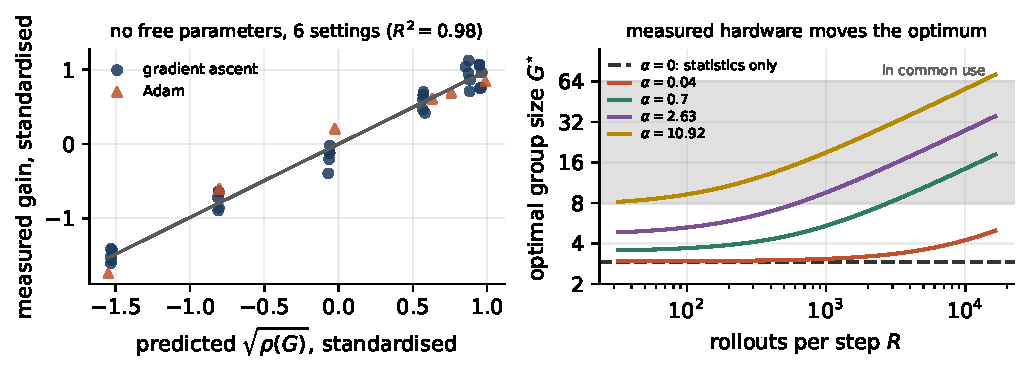
\includegraphics[width=\textwidth]{figures/allocation.pdf}
  \caption{\textbf{Left:} the efficiency $\rho(G)$ predicted from two measured traces with no
  fitted parameters, against the gain actually obtained by training at that split. Settings differ
  in run length and task, so both axes are standardised within a setting; what is pooled is the
  shape. \textbf{Right:} the optimal group size from Theorem~\ref{thm:split} at that measured noise
  ratio, against the rollout budget, for the prefill ratios $\alpha$ we measure on real hardware.
  Statistics alone say three; the hardware says the rest, and says something different for long
  prompts with short answers than for reasoning-length responses.}
  \label{fig:allocation}
\end{figure*}

Hardware fixes the rollouts per step $R = PG$; the question is how to divide them. When a group
shares its prompt's prefill, prefill is paid once per prompt and decode once per response, so a step
costs $P(c_{\mathrm{pre}} + G\,c_{\mathrm{dec}})$. Write $\alpha := c_{\mathrm{pre}}/c_{\mathrm{dec}}$
for the prefill ratio and $\beta_b := \tau_b/\mathcal{G}$, $\beta_w := \tau_w/\mathcal{G}$.

\begin{theorem}[Compute-optimal split]
  \label{thm:split}
  Under Assumption~\ref{as:regularity}, maximising the progress of
  Proposition~\ref{prop:progress} per unit of compute at fixed $R$ is equivalent to minimising
  \begin{equation}
    \label{eq:objective}
    f(G) \;=\; (\alpha + G)\Big( \frac{R}{G} + \beta_b + \frac{\beta_w}{G-1} \Big)
  \end{equation}
  over $G \in (1, \infty)$. Then:
  \begin{enumerate}
    \item[(i)] $f$ is strictly convex on $(1,\infty)$ and has a unique minimiser $G^{\star}$, which
    is the unique root of
    \begin{equation}
      \label{eq:stationary}
      \beta_b \;=\; \frac{\alpha R}{G^2} \;+\; \frac{(1+\alpha)\,\beta_w}{(G-1)^2}.
    \end{equation}
    \item[(ii)] If rollouts cost the same however they are grouped $(\alpha = 0)$, then
    \begin{equation}
      \label{eq:gstar}
      G^{\star} \;=\; 1 + \sqrt{\tau_w/\tau_b},
    \end{equation}
    exactly and independently of $R$.
    \item[(iii)] For $\alpha > 0$, $G^{\star}$ is strictly increasing in both $\alpha$ and $R$, and
    \begin{equation}
      \label{eq:gstar-cost}
      G^{\star} \;\to\; 1 + \sqrt{(1+\alpha)\,\tau_w/\tau_b}
      \quad\text{as}\quad \alpha R/G^2 \to 0 .
    \end{equation}
    \item[(iv)] The optimal integer group size is $\lfloor G^{\star}\rfloor$ or
    $\lceil G^{\star}\rceil$.
  \end{enumerate}
\end{theorem}

\begin{proof}
  By Proposition~\ref{prop:progress}, total progress under a compute budget $C$ is proportional to
  $\sqrt{N_{\mathrm{s}}\rho}$ with $N_{\mathrm{s}} = C/\big(P(c_{\mathrm{pre}} + Gc_{\mathrm{dec}})\big)$,
  so
  $N_{\mathrm{s}}\rho \propto \big[(\alpha+G)(P + \Bcrit(G))\big]^{-1}$
  using \eqref{eq:efficiency}. Substituting $P = R/G$ and
  $\Bcrit(G) = \beta_b + \beta_w/(G-1)$ gives \eqref{eq:objective}, and maximising
  $N_{\mathrm{s}}\rho$ is minimising $f$.

  Expanding, $f(G) = \alpha R/G + G\beta_b + (1+\alpha)\beta_w/(G-1) + \text{const}$, whence
  \begin{equation*}
    f''(G) = \frac{2\alpha R}{G^3} + \frac{2(1+\alpha)\beta_w}{(G-1)^3} > 0
    \qquad \text{on } (1,\infty),
  \end{equation*}
  so $f$ is strictly convex. Since $f'(G) \to -\infty$ as $G \downarrow 1$ and
  $f'(G) \to \beta_b > 0$ as $G \to \infty$, $f'$ has a unique zero, which is
  \eqref{eq:stationary}. This proves (i).

  For $\alpha = 0$ the first term of \eqref{eq:stationary} vanishes and the condition reduces to
  $\beta_b = \beta_w/(G-1)^2$, giving \eqref{eq:gstar}; $R$ has dropped out, proving (ii).
  Writing \eqref{eq:stationary} as $\Xi(G,\alpha,R) = 0$ with
  $\Xi := \beta_b - \alpha R/G^2 - (1+\alpha)\beta_w/(G-1)^2$, we have
  $\partial_G \Xi > 0$ at the root while $\partial_\alpha \Xi < 0$ and $\partial_R \Xi < 0$, so
  the implicit function theorem gives $\partial G^{\star}/\partial\alpha > 0$ and
  $\partial G^{\star}/\partial R > 0$. Dropping the $\alpha R/G^2$ term from
  \eqref{eq:stationary} leaves $\beta_b = (1+\alpha)\beta_w/(G-1)^2$, which is
  \eqref{eq:gstar-cost}. This proves (iii). Part (iv) follows from strict convexity, since a
  strictly convex function on an interval is minimised over the integers at one of the two
  integers bracketing its real minimiser.
\end{proof}

Part (ii) is the case in which the split is purely a statistical question, and there the answer is
one plus the square root of the ratio of within-prompt to between-prompt gradient noise, with no
dependence on how many rollouts the hardware affords. Both traces are measurable from a single
batch (Section~\ref{sec:estimation}), so $G^{\star}$ is an observable rather than a hyperparameter.

Part (iii) is where the economics enter, and it is the reason published recipes are not obviously
wrong. Prefill sharing pushes $G^{\star}$ up, and so does a larger rollout budget: a run with long
prompts, short responses and a large batch can have an optimum in the tens even when the purely
statistical optimum is three. Section~\ref{sec:experiments} measures $\alpha$ on real hardware and
finds it ranging from $0.04$ to $10.9$ depending only on the prompt-to-response length ratio, which
moves $G^{\star}$ over an order of magnitude. The approximation \eqref{eq:gstar-cost} that we quote
alongside is the small-batch limit and understates $G^{\star}$ badly when $R$ is large; the root of
\eqref{eq:stationary} is what should be used, and costs one line of arithmetic.

\paragraph{The optimum moves during a run.} Both $\tau_w$ and $\tau_b$ change as the policy
improves. $\E_x[p(1-p)]$ falls once a task is largely solved, while prompt-to-prompt gradient
heterogeneity falls as a model acquires a shared algorithm. Which of the two dominates is an
empirical question, and Section~\ref{sec:experiments} finds both directions in different settings.

\subsection{The step size is a drift target}

Equation \eqref{eq:drift} inverts to $\eta(D) = \sqrt{2D/(\mathcal{G} + N/P)}$, so a run can be
specified by a target drift rather than a learning rate. Learning rate, clip range and KL
coefficient are three controls acting on the single quantity $D$, which is why they interact and why
none of them transfers between settings on its own. Drift is measured in nats per token and is a
property of the policy's behaviour rather than of its parameterisation. Whether that makes it
transfer is tested in Section~\ref{sec:experiments}, and the answer has a boundary.

\subsection{What the hardware is worth}
\label{sec:hardware}

Theorem~\ref{thm:split} turns the split into a question about the serving stack as much as about
the learning problem, through the prefill ratio $\alpha = c_{\mathrm{pre}}/c_{\mathrm{dec}}$. We
measured both costs for a $0.5$B model in bfloat16 on the machine everything else ran on. The ratio
is governed almost entirely by the prompt-to-response length ratio, running from $0.04$ when a
short prompt is followed by a thousand tokens of response to $10.9$ when a thousand-token prompt is
followed by a short answer.

\begin{table*}[t]
  \centering
  \small
  \begin{tabular}{lcccc}
\toprule
$c_{\mathrm{pre}}/c_{\mathrm{dec}}$ & $R=64$ & $R=256$ & $R=1024$ & $R=8192$ \\
\midrule
0.00 & 2.9 & 2.9 & 2.9 & 2.9 \\
0.04 & 3.0 & 3.0 & 3.1 & 4.0 \\
0.70 & 3.6 & 4.0 & 5.5 & 13.1 \\
2.63 & 5.0 & 6.2 & 9.7 & 25.1 \\
10.92 & 8.7 & 11.5 & 19.2 & 51.0 \\
\midrule
\multicolumn{5}{l}{\footnotesize small-batch limit \eqref{eq:gstar-cost} --- $\alpha=0.00$: 2.9, $\alpha=0.04$: 2.9, $\alpha=0.70$: 3.5, $\alpha=2.63$: 4.6, $\alpha=10.92$: 7.6} \\
\bottomrule
\end{tabular}
  \caption{The optimum $G^{\star}$ from Theorem~\ref{thm:split}, at the noise ratio measured on our
  transformers, across measured prefill ratios and rollout budgets. Entries are the root of
  \eqref{eq:stationary}, which agrees with direct numerical minimisation of \eqref{eq:objective} to
  one part in $10^{7}$. The last row shows the small-batch limit, which is what one would quote
  from \eqref{eq:gstar-cost} alone and which understates the optimum badly at large $R$.}
  \label{tab:optimum}
\end{table*}

\begin{figure}[t]
  \centering
  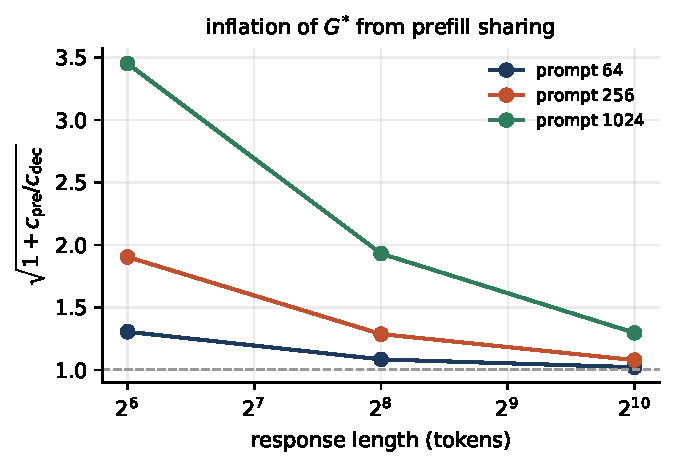
\includegraphics[width=\linewidth]{figures/cost_model.pdf}
  \caption{Measured prefill-to-decode economics on an Apple M4, as the group-size inflation implied
  in the small-batch limit. Long responses make prefill sharing almost worthless; short answers
  behind long prompts make it decisive.}
  \label{fig:cost-model}
\end{figure}

Table~\ref{tab:optimum} is the reconciliation the paper has been building towards. A purely
statistical reading of the split says three; the settings in which published recipes were developed
say otherwise, and the theorem says how much of that is justified. Long prompts with short answers
at a large batch put the optimum in the tens, which is where the recipes are. Reasoning-length
responses, where the response dwarfs the prompt, put it back at three to four, and there a group of
sixteen is spending most of its budget on responses that a second prompt would have used better.
The disagreement between a recipe and this analysis is therefore not evidence against either: it
identifies the regime the recipe came from.

\subsection{What transfers when the batch size changes}

The sharpest consequence of the drift model is a statement about transfer. A run tuned by learning
rate is tuned in a unit that depends on the batch through $\mathcal{G} + N/P$; a run tuned by drift
is not. Table~\ref{tab:transfer} sweeps both parameterisations at four batch sizes and reports what
it costs to carry the value tuned at the smallest batch to the others.

\begin{table*}[t]
  \centering
  \begin{tabular}{lcccc}
\toprule
prompts per step $P$ & 8 & 16 & 32 & 64 \\
\midrule
best step size $\eta^{*}$ & 0.0417 & 0.0786 & 0.1228 & 0.1615 \\
best drift target $D^{*}$ & 5.06e-03 & 5.29e-03 & 5.15e-03 & 3.98e-03 \\
cost of transferring $\eta$ (\%) & +0.0 & -9.9 & -17.9 & -22.0 \\
cost of transferring $D^{*}$ (\%) & +0.0 & +0.0 & +0.0 & +0.0 \\
\bottomrule
\end{tabular}
  \caption{Transfer across batch size. The learning rate that is optimal at $P = 8$ loses a fifth of
  the achievable gain by $P = 64$; the drift target that is optimal at $P = 8$ remains optimal.}
  \label{tab:transfer}
\end{table*}

\begin{figure*}[t]
  \centering
  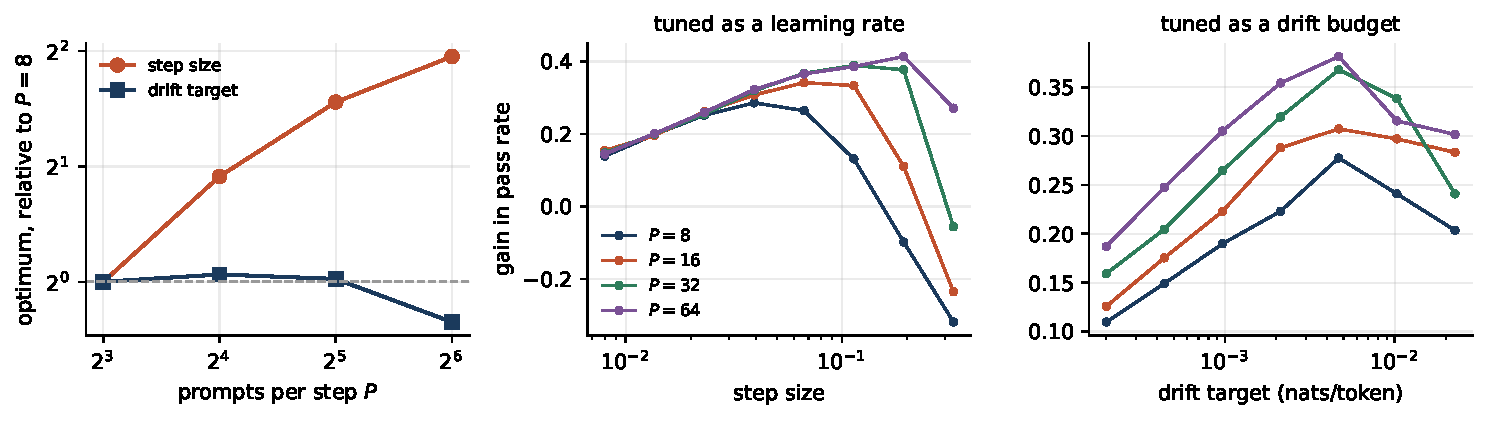
\includegraphics[width=\textwidth]{figures/transfer.pdf}
  \caption{Left: the optimum of each parameterisation relative to its value at $P = 8$. Centre and
  right: the sweeps themselves. The learning-rate optimum moves; the drift optimum does not.}
  \label{fig:transfer}
\end{figure*}

The single-step drift model accounts for part of the movement in $\eta^{*}$ and not all of it: the
coefficient $\mathcal{G} + N/P$ measured at the initial policy predicts a smaller shift than the one
observed over a full run. The coefficient keeps moving as the policy improves, so a controller that re-reads it tracks the
optimum while a learning rate fixed in advance cannot.

\subsection{Measuring the noise scales in Adam's metric}
\label{sec:adam}

Everything above is under plain gradient ascent, where the update is the gradient and the noise can
be read in the parameter metric. Real runs use Adam, which moves in a different metric and is scale
invariant, so the theory only carries over if the noise is measured after preconditioning. Repeating
the sweep under both optimisers gives Table~\ref{tab:adam}.

\begin{table*}[t]
  \centering
  \begin{tabular}{lcccccccc}
\toprule
gain by group size & 2 & 4 & 8 & 16 & 32 & 64 & measured $G^{\\star}$ & $R^2$ \\
\midrule
gradient ascent & +0.409 & +0.413 & +0.390 & +0.333 & +0.300 & +0.250 & 2.94 & 0.992 \\
Adam & +0.519 & +0.527 & +0.514 & +0.492 & +0.447 & +0.384 & 3.42 & 0.969 \\
\bottomrule
\end{tabular}
  \caption{The same sweep under gradient ascent and under Adam. The optimum is at $G = 4$ for both,
  and the predicted curve explains the measured one about as well. The measured $G^{\star}$ for Adam is
  taken in Adam's own metric, which takes some care -- see below.}
  \label{tab:adam}
\end{table*}

The law survives, but measuring in Adam's metric required fixing two things, and both are
consequences of the preconditioner being an estimated quantity rather than a fixed one.

First, a probe run at a frozen policy starts with an empty second-moment estimate, so there is no
metric to measure in yet. Priming it -- running the optimiser's state forward on real batches with
a zero step size, so the policy does not move -- gives the preconditioner a real run would have.

Second, and less obviously, dividing by $\sqrt{v}$ is unbounded. Coordinates that rarely receive
gradient have a tiny second moment, which is harmless for the update, since Adam's update is
bounded by construction, but ruinous for an inner product between two noisy gradients: those
coordinates dominate it. Measured this way the estimator returned $\tau_b < 0$ and an inverted
efficiency curve. Flooring the second moment at a fraction of its own mean before dividing fixes
it, and the result is insensitive to where the floor is put: over three orders of magnitude in the
floor, the measured $G^{\star}$ moves only from $3.51$ to $3.15$, against an observed optimum of $4$.
Without a floor the same measurement reports $11.9$.

This is the one place where our quantities need care that the plain-gradient case does not. The
working rule is to instrument the update rather than the gradient, and to floor the preconditioner
before inverting it.

\subsection{A prospective test, and where the drift target stops transferring}
\label{sec:recipe}

Everything so far tunes one quantity at a time on the setting it is measured on. The stronger test
is prospective: fix a setting the method has never seen, let the probe choose $G$ before any
training happens, and check afterwards whether it chose well. We moved to a held-out setting with
four times the rollout budget, eight times the corpus and a different seed. The probe reported
$G^{\star} = 3.1$, so the recipe took $G = 4$; the comparison is against $G = 16$, which is what a
default recipe would use.

\begin{table}[t]
  \centering
  \small
  \begin{tabular}{lcc}
\toprule
best achievable gain & $G = 4$ & $G = 16$ \\
\midrule
tuning a learning rate & +0.4947$^{\ast}$ & +0.4780$^{\ast}$ \\
tuning a drift target & +0.4431 & +0.3989 \\
predicted efficiency $\rho$ & 0.815 & 0.674 \\
\bottomrule
\end{tabular}
  \caption{Best achievable gain at the held-out setting, crossing the group size the probe selected
  against the group size a default recipe would use, under both ways of setting the step. Starred
  entries sit at the edge of their grid and are lower bounds. The probe's choice wins under both.}
  \label{tab:diagnosis}
\end{table}

\textbf{The prospective choice was right.} $G = 4$ beats $G = 16$ under both parameterisations.
Under drift control, where the step size is held to the same behavioural budget in both arms and so
cannot confound the comparison, it wins by $11.1\%$ against a predicted
$\sqrt{\rho_4/\rho_{16}} - 1 = 10\%$.

\textbf{The drift target transfers across the group size exactly.} Both group sizes put their
optimum at the same drift target, $1.45 \times 10^{-3}$. Changing how the budget is split does not
change how far the policy should move per update, which is what a behavioural unit ought to do.

\textbf{It does not transfer across this change of budget.} The tuning setting's optimum was
$3.19 \times 10^{-3}$, a factor of $2.2$ away, and carrying it over costs $20\%$ of the achievable
gain. Earlier the same target held to within $5\%$ across a fourfold change in batch size and
$21\%$ across an eightfold one. A sixteenfold change in prompts per step, combined with a fourfold
change in rollout budget, is past where a single number holds. We found this the hard way: packaging
the two together and carrying both to the held-out setting lost to the default by $28.9\%$ (paired
$t = -3.01$ over $32$ runs), and Table~\ref{tab:diagnosis} is what attributes that loss to the drift
target rather than to the group size.

\textbf{A constant drift target is not the right schedule.} At both group sizes a tuned constant
learning rate beat the best constant drift, with its optimum at the edge of the grid. A fixed
learning rate produces a drift that changes over a run as the gradient statistics change, and that
this wins says the optimal drift trajectory is not flat. The unit appears to be right and the
schedule is not, which is the most concrete thing this paper leaves open.
